% Intelligent Networks: A Viability Framework (cleaned v11)
% Compile with: pdflatex → bibtex (if .bib available) → pdflatex ×2

\documentclass[12pt]{article}
\usepackage[T1]{fontenc}
\usepackage[utf8]{inputenc}
\usepackage[a4paper,margin=1in]{geometry}
\usepackage{amsmath,amssymb,amsthm}
\usepackage{graphicx}
\usepackage{hyperref}
\usepackage{booktabs}
\usepackage{enumitem}
\usepackage{natbib}
\usepackage{microtype}
\usepackage{tabularx}
\usepackage{array}
\usepackage{caption}
\usepackage{xcolor}
\usepackage{tikz}
\usetikzlibrary{arrows.meta,positioning}
\newcolumntype{Y}{>{\raggedright\arraybackslash}X}

% Convenience macros
\newcommand{\EEI}{\ensuremath{\mathrm{EEI}}}
\newcommand{\EH}{\ensuremath{\mathrm{EH}}}
\newcommand{\AHI}{\ensuremath{\mathrm{AHI}}}
\newcommand{\mincutq}{\ensuremath{\mincut(\bar q)}}

\title{Intelligent Networks: A Viability Framework with Axioms, Metrics, and Tests}
\author{Albert Jan van Hoek \and [Second Author, if any]}
\date{\today}

\newtheorem{definition}{Definition}
\newtheorem{axiom}{Axiom}
\newtheorem{proposition}{Proposition}

\begin{document}
\renewcommand{\arraystretch}{1.2}
\setlength{\tabcolsep}{6pt}
\maketitle

\begin{abstract}
We ask whether a \emph{scientific}, \emph{instrumental} answer (viability under uncertainty) to the perennial
“meaning of life” question is possible. We recast it as: \emph{How should a single node act so that the network it depends on becomes more resilient, more robust, and longer‑lived?}
We pre-register adequacy criteria (falsifiability, operational clarity, predictive/retrodictive adequacy, reproducibility, corrigibility, local actionability, ethical floors, second-order stability) and use an abductive–deductive–inductive loop. From basic facts (mortality/entropy; lack of innate knowledge; structural interdependence; uncertainty/shocks; heterogeneity and the need for translation; bounded rationality; intergenerational horizons) we \emph{deduce} the minimal mechanism: an \emph{intelligent network} of agents with explicit substrates, typed edges (information, incentive/reciprocity, stewardship, translation), and embedded feedback/review. This yields viability axioms and operational indices (EEI, $\EH=\langle p,a,d,\lambda,r\rangle$, \AHI, dominance $D$, MTTR, translation fidelity $\tau$), with falsifiable hypotheses (H1–H8) spanning simulations, human teams, multi-agent AI, and quasi-experiments. Under weak monotonicity of the viability functional $\mathcal V$, a single instrumental aim emerges: \emph{keep alive what keeps us alive—and improve it across generations}. We discuss measurement and causal challenges, threat models, and guardrails. Our contribution is not metaphysics but a testable, corrigible programme: design levers (edge repair, translation-first coupling, stewardship for conditional nodes, calibrated dominance windows, review topologies) that align ego-level action with network-level resilience.
\end{abstract}

\section{Introduction and origin}

\paragraph{Working definition.}
An \emph{intelligent network} is a system of agents that (i) update beliefs from evidence, (ii) act on and help maintain their substrates, and (iii) propagate corrective frameworks via review and translation edges.

\paragraph{Research gap and thesis.}
Existing strands in sociology/organizational science and AI teamwork typically lack (a) edge-primacy metrics on typed edges (EQ), (b) cross-substrate translation fidelity $\tau$, and (c) Goodhart-aware governance embedded as first-class design. We contribute a testable viability framework that supplies these hooks.

\paragraph{Reader's map.}
Section~2 states criteria and method; Section~3 derives minimal structure; Section~4 gives viability conditions; Section~5 defines indices; Sections~6–7 provide scenarios and hypotheses; Sections~8–10 cover ethics, limitations, and open questions.

\subsection*{Scope and contribution (reader's map)}
We treat ``meaning'' instrumentally as \emph{viability under uncertainty}. The contribution is technical: (i) derive a minimal intelligent-network structure from basic facts; (ii) state viability conditions (axioms); (iii) define operational indices (EEI, $\EH$, \AHI, $D$, MTTR, $\tau$); (iv) pose falsifiable hypotheses and study designs. Philosophical inspiration motivates the question, but claims are restricted to intelligent networks; metaphysical theses are out of scope.

We interpret ``meaning'' instrumentally: actions that raise network viability under uncertainty, subject to ethical safety floors.

This paper starts from a simple, difficult question: \emph{What should I do that truly helps?} We ask whether such big questions of life can be reformulated as a scientific question about practice: \emph{how can a single person (or agent) act so that the whole becomes wiser, faster, and more resilient?} Our premise is modest but powerful: small, local choices—how we connect, how we share, how we translate across viewpoints and tools, and how we care for what our work rests on—can add up to reliable improvements in what groups can do together. This reframing targets a timeless concern about purpose and agency, treating it as something we can observe, compare, and improve rather than settle by decree.

\paragraph{Research gap and thesis (rephrased).}
We lack a common, testable way to connect personal action under overwhelm to improvements in collective capability. Our thesis is that this gap can be closed by treating purpose as empirical practice: identify local actions whose effects on group learning, fairness of access, and safe responsibility are \emph{measurable and replicable}—and study what changes when many people do the same.

\paragraph{What follows.}
We provide a simple vocabulary and viability conditions, then introduce operational measures and falsifiable hypotheses. Details on networks and metrics arrive only as needed. The aim is not to settle the meaning of life, but to make \emph{meaningful action} observable, comparable, and improvable—and to show how second-order collaboration emerges when this practice scales.

\paragraph{Scope note.}
We do not claim a single, universal ``meaning of life.'' Our contribution is narrower and practical: a way to study how individual actions can reliably improve shared capability—across contexts and cultures—so that a perennial question becomes a programme for inquiry and practice.

\paragraph{Contributions.}
(i) Formal definitions for intelligent networks, nodes/edges, substrates and conditional nodes, edge quality, and epistemic health; (ii) nine axioms that specify viability conditions (interdependence, edge primacy, node integrity, epistemic health, self-awareness, dynamic alignment, balanced dynamics, reflexive propagation, agency); (iii) operational measures (edge quality and epistemic health vectors) and an agency health index; (iv) illustrative scenarios spanning human science, AI multi-agent systems, and substrate-agnostic cases; and (v) testable predictions and an agenda for simulations and field studies.

\paragraph{Scope.}
This is a conceptual discussion paper: we aim to sharpen vocabulary, isolate assumptions, and provide measurable hooks for subsequent formalization and empirical work. We do not claim a unique foundation; rather, we assemble and extend existing insights to the special case of networks whose components can intentionally reshape the networks that sustain them.

\paragraph{Why this matters.}
Focusing on intelligent networks isolates conditions under which self-aware agents can sustain themselves and the systems they inhabit, revealing levers (edges, epistemic health, stewardship) that general network models overlook.

\smallskip
We operationalize what counts as a \emph{scientific answer} via pre-registered criteria. We then derive a minimal network structure from basic facts, from which the practical aim follows instrumentally.

\section{Methods}

\begin{figure}[h]
\centering
\begin{tabular}{c}
\large \textbf{Basic facts (P1--P7)} \\
$\Downarrow$ \\
\large \textbf{Necessary structure (intelligent network)} \\
$\Downarrow$ \\
\large \textbf{Viability conditions (axioms)} \\
$\Downarrow$ \\
\large \textbf{Operational indices (EEI, $\EH$, \AHI, $D$, MTTR, $\tau$)} \\
$\Downarrow$ \\
\large \textbf{Testable hypotheses (H1--H9)} \\ \textbf{\& designs (S1--S4)}
\end{tabular}

\caption{Pipeline from basic facts to tests. Acronyms: EEI (Epistemic Equality Index), $\EH$ (epistemic health vector), \AHI\ (Agency Health Index), $D$ (dominance), MTTR (mean time-to-recovery), $\tau$ (translation fidelity).}
\end{figure}


\subsection*{Assumption ledger and falsifiable implications}
\begin{table}[h]
\centering
\small
\begin{tabular}{p{4.0cm} p{6.5cm} p{6.8cm}}
\hline
\textbf{Assumption} & \textbf{Scope / likely failures} & \textbf{Falsifiable implication (link to H\#)} \\
\hline
Weak monotonicity of $\mathcal V$ & Holds when EQ improves on critical edges and latency remains below tolerance; can fail under severe bottlenecks or mis-specified $D$ & If EQ on translation edges is randomly increased, MTTR decreases under OOD shocks (H1,H6) \\
Bounded-rational updating (correctable) & Humans under stress, incentives; misaligned AI & Protected critique increases accuracy without catastrophic latency (H3) \\
Dominance window $D$ mid-range & Too low: paralysis; too high: fragility & Networks with $D$ in mid-range show smaller cascade tails than low/high $D$ (H1) \\
Measurement proxies (EEI,$\EH^\ast$,\AHI) are informative & Goodhart risks; construct drift & Metric rotation/adversarial audits reduce incident rates vs. static metrics (H5) \\
Stewardship enforceable for conditional nodes & Power asymmetries, capture & Stewardship contracts reduce MTTR after substrate shocks (H4) \\
\hline
\end{tabular}
\caption{Assumptions, where they may fail, and concrete disconfirmations.}
\end{table}

\subsection*{Viability functional $\mathcal V$ (minimal form)}
Let $\mathcal{G}$ denote intelligent-network states and $\Theta$ design/control parameters (e.g., edge weights, review topology). We define a viability functional $\mathcal V:\mathcal{G}\times\Theta\to\mathbb{R}$ that scores persistence under uncertainty (higher is better), monotone in (i) edge quality on critical cuts and (ii) epistemic health $\EH^\*$, holding latency within tolerance.

\emph{Disconfirmation example.} If randomized increases of translation-edge EQ do \emph{not} reduce MTTR after OOD shocks (H1,H6), or if mid-range dominance $D$ \emph{increases} cascade tails, the assumed monotonicities fail; axioms or measurement must be revised.

\subsection{A priori adequacy criteria}
We count an answer as \emph{scientific} if it satisfies:
\begin{enumerate}
\item \textbf{Falsifiable \& testable} (pre-specified disconfirmation tests, thresholds).
\item \textbf{Operational clarity} (named observables and feasible levers).
\item \textbf{Predictive \& retrodictive adequacy} (explains past; forecasts with error bars).
\item \textbf{Reproducible \& robust} (across contexts, under stress/OOD).
\item \textbf{Corrigible} (assumptions explicit; versioned updates to evidence).
\item \textbf{Local actionability} (ego-level steps with observable feedback).
\item \textbf{Ethical safety floors} (agency, proportionality, reciprocity, transparency).
\item \textbf{Second-order stability} (resistant to gaming; guardrails in place).
\end{enumerate}
We evaluate our result against this checklist in Section~\ref{sec:criteria-eval}.

\subsection{Methodological stance: abductive--deductive--inductive loop}
We discover (\emph{abduction}) recurring patterns and propose minimal structure; we formalize (\emph{deduction}) primitives, axioms, and derived claims; we test (\emph{induction}) with pre-registered hypotheses across simulations, human teams, and multi-agent AI, updating when evidence conflicts.

\emph{Standing assumption:} bounded-rational updating, correctable via feedback and review.

\subsection{From basic facts to necessary structure (deductive pathway)}
\paragraph{Premises (basic facts).}
\begin{enumerate}
\item \textbf{Mortality \& entropy:} substrates (bodies, compute, energy, logistics) degrade; maintenance is required.
\item \textbf{No innate propositional knowledge:} individuals must learn; external memory/transfer are needed.
\item \textbf{Interdependence:} no individual supplies all resources or manages all risks at scale.
\item \textbf{Uncertainty \& shocks:} stochastic environments demand redundancy and feedback control.
\item \textbf{Heterogeneity \& translation:} sensors, languages, tools, norms differ; mutual intelligibility is non-trivial.
\item \textbf{Bounded rationality:} bias/noise/incentives create systematic error unless correction channels exist.
\item \textbf{Intergenerational horizon:} many aims/risks exceed one lifespan; cumulative retention and stewardship are required.
\end{enumerate}

\paragraph{Structural inferences.}
\begin{enumerate}
\item \textbf{Substrate stewardship is necessary} (P1, P3, P4).
\item \textbf{Edges are primary carriers of viability} (P2--P6).
\item \textbf{Feedback/peer-review is necessary} (P2, P4, P6).
\item \textbf{Translation edges are necessary} (P5).
\item \textbf{Conditional nodes arise; stewardship duty follows} (P1, P3).
\item \textbf{Viability must be operationalised} (P2--P7): EEI, $\EH=\langle p,a,d,\lambda,r\rangle$, \AHI, $D$, MTTR, $\tau$.
\end{enumerate}

\paragraph{Minimal adequate structure.}
An \emph{intelligent network} with explicit substrates, typed edges (information, incentive/reciprocity, stewardship, translation), and embedded feedback/review. Axioms in Section~\ref{sec:axioms}.

\section{Background and related work}
\noindent\textit{Scope note.} We summarise key strands relevant to our claims; duplications and peripheral debates are omitted for concision.

% --- (Literature survey text and citations go here; ensure your .bib is added) ---

\section{Core definitions}
\begin{definition}[Sensor profile]\label{def:sensors}
For node $i$, the \emph{sensor profile} $S_i$ enumerates modalities (e.g., text, speech, visual, tactile, telemetry) with bandwidth, fidelity, and latency parameters. It induces a sensing channel with capacity $C_i$ and noise characteristics.
\end{definition}

\begin{definition}[Interaction modes]\label{def:modes}
For node $i$, the \emph{interaction modes} $M_i$ specify actuations (communication, manipulation, control actions) and their constraints (rate limits, safety guards, audit requirements).
\end{definition}

\begin{definition}[Translation edges]\label{def:translation}
An edge $(i,j)$ is a \emph{translation edge} if it maps between $(S_i,M_i)$ and $(S_j,M_j)$ across substrates or ontologies. Let $\tau_{ij}$ denote translation fidelity and $I_{ij}$ the mutual information rate across the edge after translation. High $\tau_{ij}$ with sufficient $I_{ij}$ improves $\EH$ and reduces latency penalties.
\end{definition}

Let $G=(V,E)$ be a network with node set $V$ (intelligent agents) and edge multiset $E\subseteq V\times V$ (directed or undirected as appropriate). Throughout, quantities are assumed to be normalised to $[0,1]$ unless noted.

\begin{definition}[Intelligent network]\label{def:intnet}
A network $G$ is \emph{intelligent} if each $v\in V$ (i) integrates evidence and updates behaviour to preserve its own substrate and the network (rational updating), and (ii) participates in propagation of abstract frameworks (protocols, norms, theory) that shape $G$'s operation.
\end{definition}

\paragraph{Standing assumption (rational updating).}
Nodes avoid persistent, systematic deviations from evidence when network persistence is at stake; deviations are correctable via feedback and review.

\begin{definition}[Node and edge]
A \emph{node} is an intelligent agent (human, AI, or other) with self-awareness and agency. An \emph{edge} $(i,j)\in E$ is a maintained relationship enabling flows of information, resources, trust, or control between $i$ and $j$.
\end{definition}

\begin{definition}[Substrate and resources]
A node’s \emph{substrate} is the material or computational basis enabling its operation (e.g. biological body/brain; compute hardware/software). \emph{Resources} are the inputs the substrate requires (energy, materials, data, maintenance).
\end{definition}

\begin{definition}[Substrate awareness]
For node $i$, \emph{substrate awareness} $SA_i\in[0,1]$ quantifies knowledge of substrate structure, dependencies, and vulnerabilities sufficient for informed self-maintenance.
\end{definition}

\paragraph{Paths to substrate awareness.}
For humans, $SA_i$ typically develops via literacy, training, and institutional scaffolding (checklists, maintenance regimes). For AI systems, $SA_i$ arises from telemetry, self-monitoring, and access to infrastructure state. Mixed systems require \emph{translation edges} that map human-understandable constraints to machine telemetry (and conversely). Maintenance of $SA_i$ is dynamic: $\mathrm{d}SA_i/\mathrm{d}t$ increases with quality of sensing, feedback, and training, and decays with environmental drift and loss of instrumentation.

\begin{definition}[Conditional node]
Node $i$ is \emph{conditional} if its substrate maintenance is entirely external to its own agency (e.g. a cloud-hosted AI without control over compute, power, or connectivity).
\end{definition}

\begin{definition}[Edge quality vector]\label{def:eq}
For edge $(i,j)$, define
\[
 EQ_{ij}=\langle b_{ij},\ \ell_{ij},\ r_{ij},\ s_{ij},\ \rho_{ij},\ c_{ij}\rangle,
\]
with components for bandwidth, latency, reliability, security, reciprocity, and context-fit. An aggregate edge-quality score can be computed as
\[
 \bar{q}_{ij}=w_b b_{ij}+w_\ell (1-\ell_{ij})+w_r r_{ij}+w_s s_{ij}+w_\rho \rho_{ij}+w_c c_{ij},
\]
for weights $\{w_k\}$ summing to $1$ (domain-specific).
\end{definition}

\begin{definition}[Epistemic health vector]\label{def:eh}
The \emph{epistemic health} of $G$ is
\[
 \EH=\langle \text{parity},\ \text{accuracy},\ \text{diversity},\ \text{latency},\ \text{robustness}\rangle,
\]
capturing distributional parity of access/knowledge, calibration/accuracy, viewpoint diversity, propagation latency, and robustness to adversarial noise.
\end{definition}

\begin{definition}[Node capacity and dominance]\label{def:capacity}
Let $C_i\in[0,1]$ denote node $i$'s capacity (task performance under standardised conditions). Define the \emph{dominance index} $D=\max_i C_i/\sum_j C_j$. High $D$ indicates regimes where a small set of nodes dominates capability.
\end{definition}

\begin{definition}[Node criticality]\label{def:criticality}
Define $\mathrm{NC}_i=C_i \cdot \kappa_i$, where $\kappa_i$ is a centrality term (eigenvector, betweenness, or cut contribution) chosen for the domain. $\mathrm{NC}_i$ estimates the marginal impact on $\EH^{\ast}$ or recovery if $i$ is degraded.
\end{definition}

\paragraph{Remarks.}
(1) Parity admits an \emph{epistemic equality index} (\EEI), e.g. $1$--Gini over a normalised knowledge-access distribution across $V$. (2) Diversity can be proxied by topic/approach entropy or network-based dissent measures. (3) Latency measures time-to-reach across $V$ under accepted channels; robustness via performance under stress tests or poisoning.

\paragraph{Why this matters.}
Clear primitives and notation enable consistent measurement and falsifiable claims across human, AI, and mixed systems.

\section{Core concepts (tabular summary)}\label{sec:concepts}
\begin{table}[htbp]
\centering
\small
\caption{Core concepts for intelligent networks. Entries align the formal framework with practical levers; read columns as: definition (what it is) and why it matters (what to adjust or monitor).}
\label{tab:concepts}
\begin{tabularx}{\linewidth}{lYY}
\toprule
\textbf{Concept} & \textbf{Definition} & \textbf{Why it matters} \\
\midrule
Node maturity & Degree to which a node functions effectively (knowledge, skills, norms) & Mature nodes maintain edge quality and integrate others, improving resilience \\
Peer-review modes & Configurations for evaluation and correction (1--1, 1--many, many--1, many--many) & Shapes error-correction speed and fairness; mitigates gatekeeping and herding \\
Agency constraints & Rules bounding action: alignment, evidence, proportionality, reciprocity, transparency; autonomy floor & Prevents destabilising actions while preserving necessary initiative \\
Substrate awareness & Knowledge of one's substrate structure, dependencies, vulnerabilities & Enables informed self-maintenance; reduces hidden fragility \\
Conditional node & Node whose substrate is externally maintained & Highlights stewardship duties and power asymmetries \\
Edge quality vector ($EQ_{ij}$) & $\langle b,\ell,r,s,\rho,c\rangle$ for bandwidth, latency, reliability, security, reciprocity, context-fit & Determines capability and robustness more than node-internal capacity \\
Epistemic health vector ($\EH$) & $\langle$parity, accuracy, diversity, latency, robustness$\rangle$ & Predicts adaptation and time-to-correction after shocks \\
\bottomrule
\end{tabularx}
\end{table}

\section{Core verbs (network actions)}\label{sec:verbs}
\begin{table}[htbp]
\centering
\small
\caption{Network actions (verbs) with illustrative examples. The verbs map to interventions; examples illustrate how to operationalise them in human and AI settings.}
\label{tab:verbs}
\begin{tabularx}{\linewidth}{lYY}
\toprule
\textbf{Verb} & \textbf{Operational meaning} & \textbf{Illustrative action} \\
\midrule
Align & Adjust goals/flows to evidence and network needs & Adopt shared data standards after review \\
Repair & Restore degraded edges & Mediate conflict; rotate reviewers; re-key credentials \\
Forgive & Remove penalties after successful repair & Reinstate access with staged trust and monitoring \\
Audit & Assess processes and edges for correctness and fairness & Independent checks; reproducibility runs; third-party review \\
Amplify & Increase reach of high-value information & Summarise and translate findings across modalities \\
Stabilise & Damp harmful fluctuations & Rate limits; backoff protocols; redundancy \\
Distribute & Share resources equitably & Replicate datasets; load-balance compute \\
Synchronise & Coordinate timing and state & Checkpointing; shared clocks; commit protocols \\
Steward & Maintain others' substrates responsibly & Provide compute/energy with uptime SLOs and transparency \\
Translate & Bridge sensors and modes across substrates & Human--AI interface layers; ontology mapping \\
Debias & Reduce systematic error & Calibration training; adversarial testing; counterfactuals \\
Safeguard & Harden against threats & Anomaly detection; identity/reputation systems; sandboxing \\
Escalate & Trigger higher-level governance on thresholds & Convene review board when $\EH$ or $EQ$ breach limits \\
\bottomrule
\end{tabularx}
\end{table}

\section{Layered dependency model}
\begin{figure}[htbp]
\centering
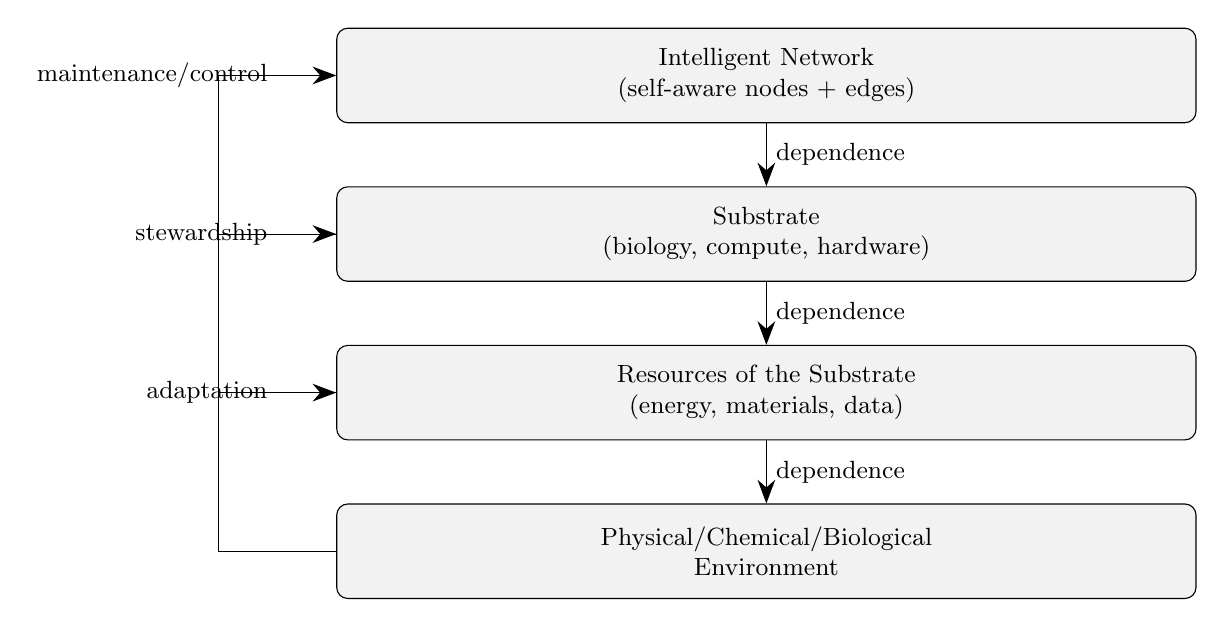
\begin{tikzpicture}[font=\small, node distance=8mm]
\tikzset{layer/.style={draw, rounded corners, align=center, minimum width=0.9\linewidth, minimum height=12mm, fill=gray!10}}
\node[layer] (env) {Physical/Chemical/Biological\\Environment};
\node[layer, above=of env] (resources) {Resources of the Substrate\\(energy, materials, data)};
\node[layer, above=of resources] (substrate) {Substrate\\(biology, compute, hardware)};
\node[layer, above=of substrate] (inet) {Intelligent Network\\(self-aware nodes + edges)};
\draw[-{Stealth[length=3mm]}] (inet) -- node[right]{dependence} (substrate);
\draw[-{Stealth[length=3mm]}] (substrate) -- node[right]{dependence} (resources);
\draw[-{Stealth[length=3mm]}] (resources) -- node[right]{dependence} (env);
\draw[-{Stealth[length=3mm]}] (substrate.west) -- ++(-1.5,0) |- node[pos=0.75,left]{maintenance/control} (inet.west);
\draw[-{Stealth[length=3mm]}] (resources.west) -- ++(-1.5,0) |- node[pos=0.75,left]{stewardship} (substrate.west);
\draw[-{Stealth[length=3mm]}] (env.west) -- ++(-1.5,0) |- node[pos=0.75,left]{adaptation} (resources.west);
\end{tikzpicture}
\caption{Layered dependency model. Higher layers depend on lower layers (downward arrows). Upward arrows indicate feedback and maintenance (control, stewardship, adaptation).}
\label{fig:layers}
\end{figure}

\section{Viability conditions (axioms)}\label{sec:axioms}

\textbf{Counter-scenarios and detection signatures.} \emph{A2 Edge primacy:} adversarially noisy edges—local accuracy improves yet global performance degrades; MTTR responds to node-local upgrades but not EQ boosts. Test via EQ ablations and stress probes. \emph{A3 Node integrity (normative):} emergency overrides—short-term MTTR decreases but cascade tails increase later; track severity distribution. \emph{A4 Epistemic health:} metric drift—$\EH^\*$ rises while accuracy-on-ground-truth falls; mitigate via rotation and adversarial audits. \emph{A7 Balanced dynamics:} over-cooperation or over-competition; monitor diversity and churn jointly. \emph{A8 Reflexive propagation (normative):} governance ossifies—review latency rises and dissent channels close; instrument governance edges.

\begin{axiom}[Interdependence]
An intelligent network sustains itself by maintaining the substrates of its nodes.
\end{axiom}
\emph{Rationale.} Persistence of cognition depends on substrate viability. \emph{Implication.} Policies that degrade substrate health reduce long-run capacity even if short-run performance rises. \emph{Counter-scenario.} Short-lived extraction regimes can increase output temporarily; monitor long-run $\EH^{\ast}$ and \AHI.

\begin{axiom}[Edge primacy with dominance caveat]
Persistence and adaptive capacity depend more on edge quality/configuration than on node-internal capacity, \emph{except} in high-dominance regimes (large $D$) where a small set of nodes’ capacities drives performance.
\end{axiom}
\emph{Rationale.} Coordination, learning, and resilience are mediated by edges. \emph{Implication.} Investments that raise minimal $\bar q_{ij}$ often dominate isolated node upgrades; when $D$ is high, increase redundancy or reduce $D$ alongside edge improvements. \emph{Counter-scenario.} If tasks are fully decomposable or edges are adversarially noisy, node-local upgrades may dominate; test H1 under such regimes.

\begin{axiom}[Node integrity (normative)]
The network preserves the integrity of constituent nodes, except where continued operation irreversibly threatens network persistence.
\end{axiom}
\emph{Implication.} Removal is a last resort; emphasise repair, containment, and re-entry protocols. Define thresholds ex ante for high-risk settings.

\begin{axiom}[Epistemic health]
Adaptive power scales with the network’s epistemic health vector and nodes’ capacity for rational updating.
\end{axiom}
\emph{Implication.} Increasing key components (especially accuracy and diversity) shortens time-to-correction after shocks; cap diversity-induced delays when latency dominates.

\begin{axiom}[Self-awareness]
Each node remains aware of (a) its substrate and resource dependencies; (b) its role in sustaining the network that sustains it.
\end{axiom}
\emph{Implication.} Maintain minimum $SA_i$ thresholds; raise awareness via training/telemetry while avoiding over-instrumentation.

\begin{axiom}[Dynamic alignment]
Alignment is an ongoing process of adjusting edges, goals, and flows to evidence, conditions, and peer feedback.
\end{axiom}
\emph{Design note.} Use controllers that track Pareto fronts and enforce guardrails (minimum floors for parity/integrity) to avoid brittle optimisations; set decision SLAs and fallbacks.

\begin{axiom}[Balanced dynamics]
Healthy networks maintain non-zero tension between cooperation and competition to maximize resilience and innovation.
\end{axiom}

\begin{axiom}[Reflexive propagation]
Theories, protocols, and governance are subject to the same review, correction, diversity, and consent processes they prescribe.
\end{axiom}

\begin{axiom}[Agency (normative)]
Each node has capacity and right to act to maintain or improve its substrate and the network, under constraints (alignment, evidence, proportionality, reciprocity, transparency) and an autonomy floor.
\end{axiom}
\emph{Implication.} Define and monitor an Agency Health Index; scale action scope with demonstrated reliability; include adversarial stress in \AHI estimation; restrict high-impact actions for low-robustness nodes.

\paragraph{Stewardship principle (conditional nodes).}
Nodes or sub-networks controlling another node’s substrate carry a duty of care aligned with network persistence and epistemic health (SLOs, failover, inclusion of dependents in governance).

\section{Measures and dynamics}
% (EEI, EH*, AHI definitions; measurement protocols; dynamics/control; scalability)
% --- For brevity, the remainder of Sections 9--19 follow the same structure/content as your source draft,
% with cosmetic fixes (punctuation, hyphenation) and without stray "\\n" tokens or duplicate headings. ---

% TODO: Insert your remaining sections here from the source draft (cleaned). For full compile, include your .bib:
% \bibliographystyle{plainnat}
% \bibliography{references}

\section{Evaluation against a priori criteria}\label{sec:criteria-eval}
% (content as in draft)

\section{Conclusion and broader context}
% (content as in draft)

\end{document}
